\documentclass[a4paper]{article}

\usepackage{amsmath}
\usepackage[english]{babel}
\usepackage[babel=true]{microtype}
\usepackage{wrapfig}
\usepackage{url}
\usepackage{mathrsfs} 
\usepackage[absolute]{textpos}
\usepackage{graphicx}
\usepackage{geometry}
\geometry{a4paper,left=40mm,right=30mm, top=3cm, bottom=3cm} 
\usepackage{subcaption}
\usepackage{float}

\newcommand{\Fermi}{\textit{Fermi} }

\begin{document}

\begin{figure}
    \begin{subfigure}{0.7\textwidth}
        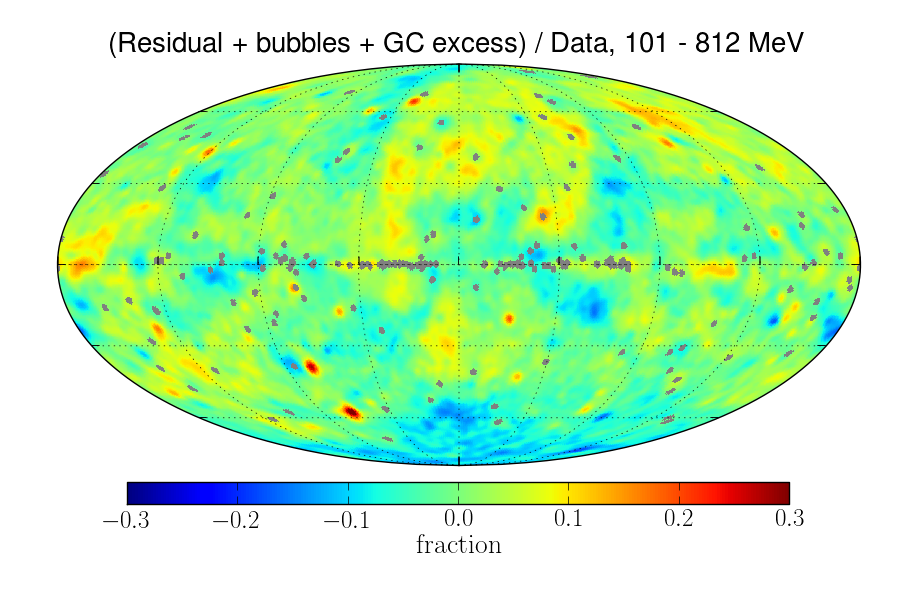
\includegraphics[width=\textwidth]{Source_refit_3FGL_40PS_resid_signal_frac_bubbles_E101-812MeV_jet}
    \end{subfigure} 
    \begin{subfigure}{0.7\textwidth}
        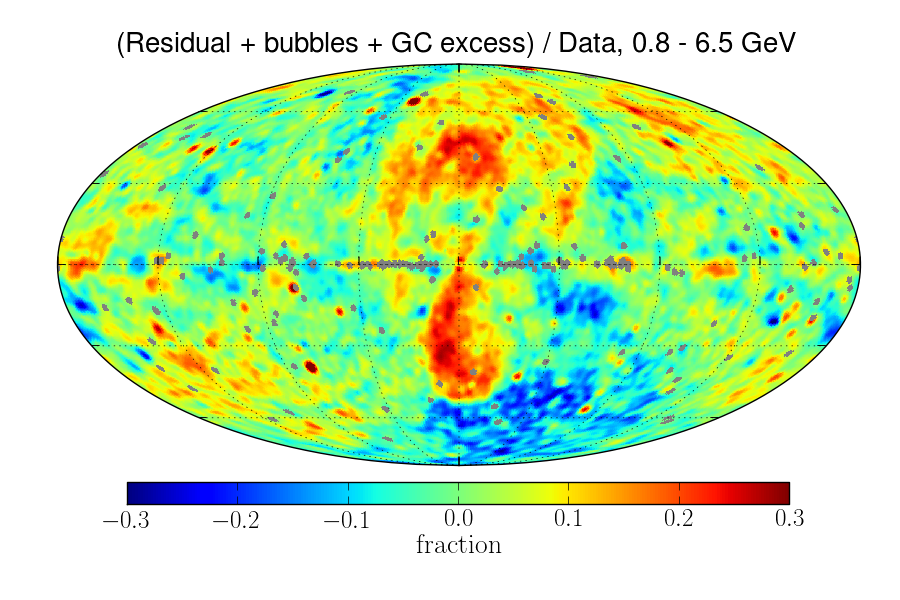
\includegraphics[width=\textwidth]{Source_refit_3FGL_40PS_resid_signal_frac_bubbles_E0p8-6p5GeV_jet}
    \end{subfigure}
    \begin{subfigure}{0.7\textwidth}
        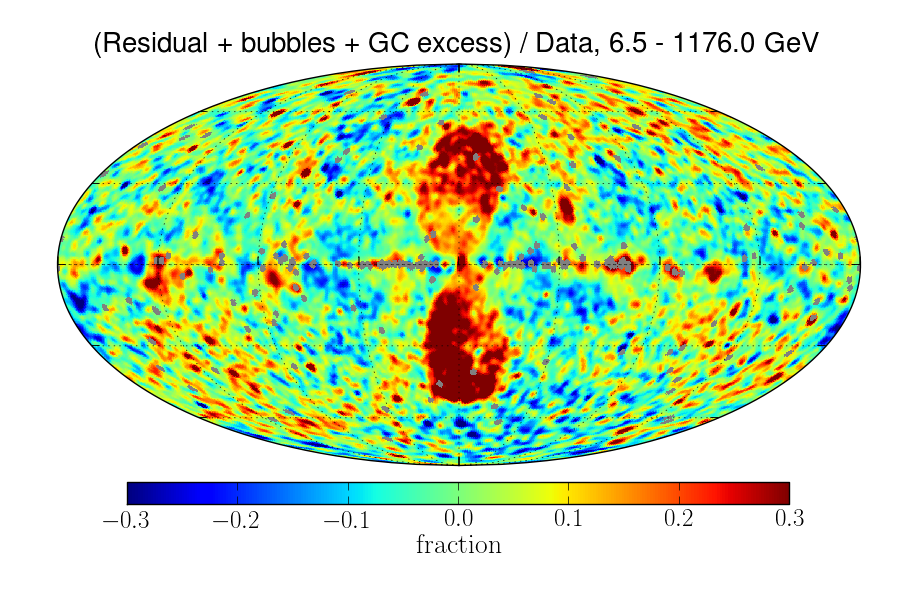
\includegraphics[width=\textwidth]{Source_refit_3FGL_40PS_resid_signal_frac_bubbles_E6p5-1176p0GeV_jet}
    \end{subfigure} 
    \caption{Mollweide maps of GALPROP full-diffusion residual in three different energy ranges}
\end{figure}


\begin{figure}
    \begin{subfigure}{0.5\textwidth}
        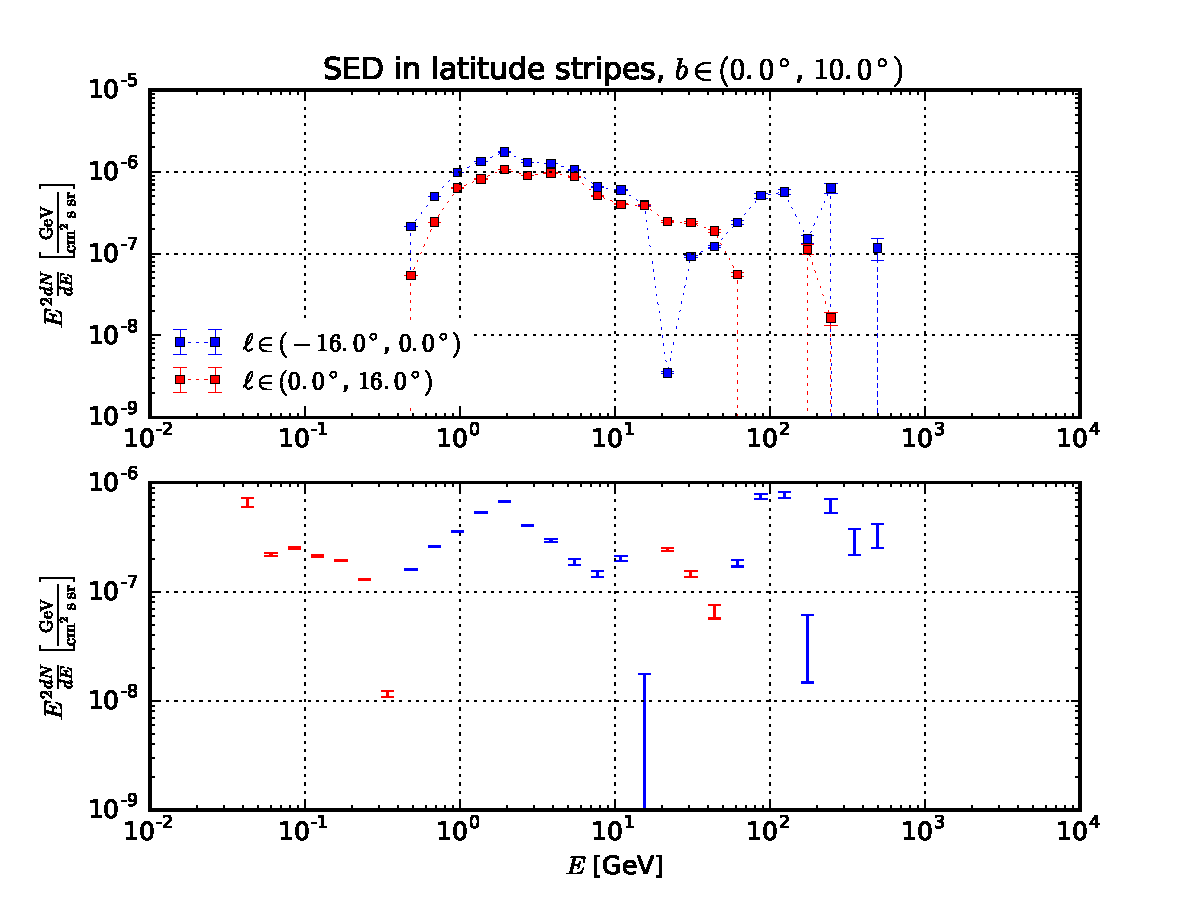
\includegraphics[width=\textwidth]{spectrum_of_top_bubble_in_lat_stripes_0-10.pdf}
    \end{subfigure} 
    \begin{subfigure}{0.5\textwidth}
        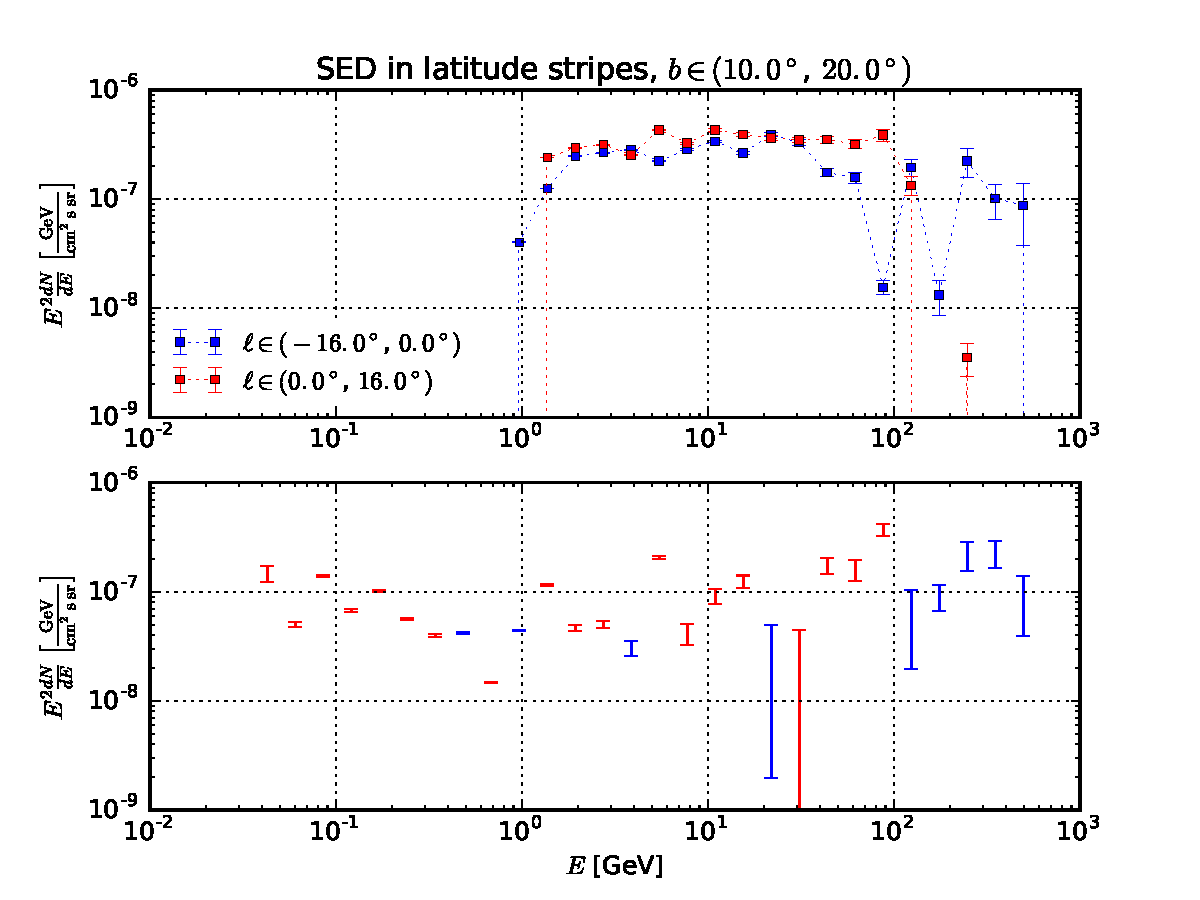
\includegraphics[width=\textwidth]{spectrum_of_top_bubble_in_lat_stripes_10-20.pdf}
    \end{subfigure}
    \begin{subfigure}{0.5\textwidth}
        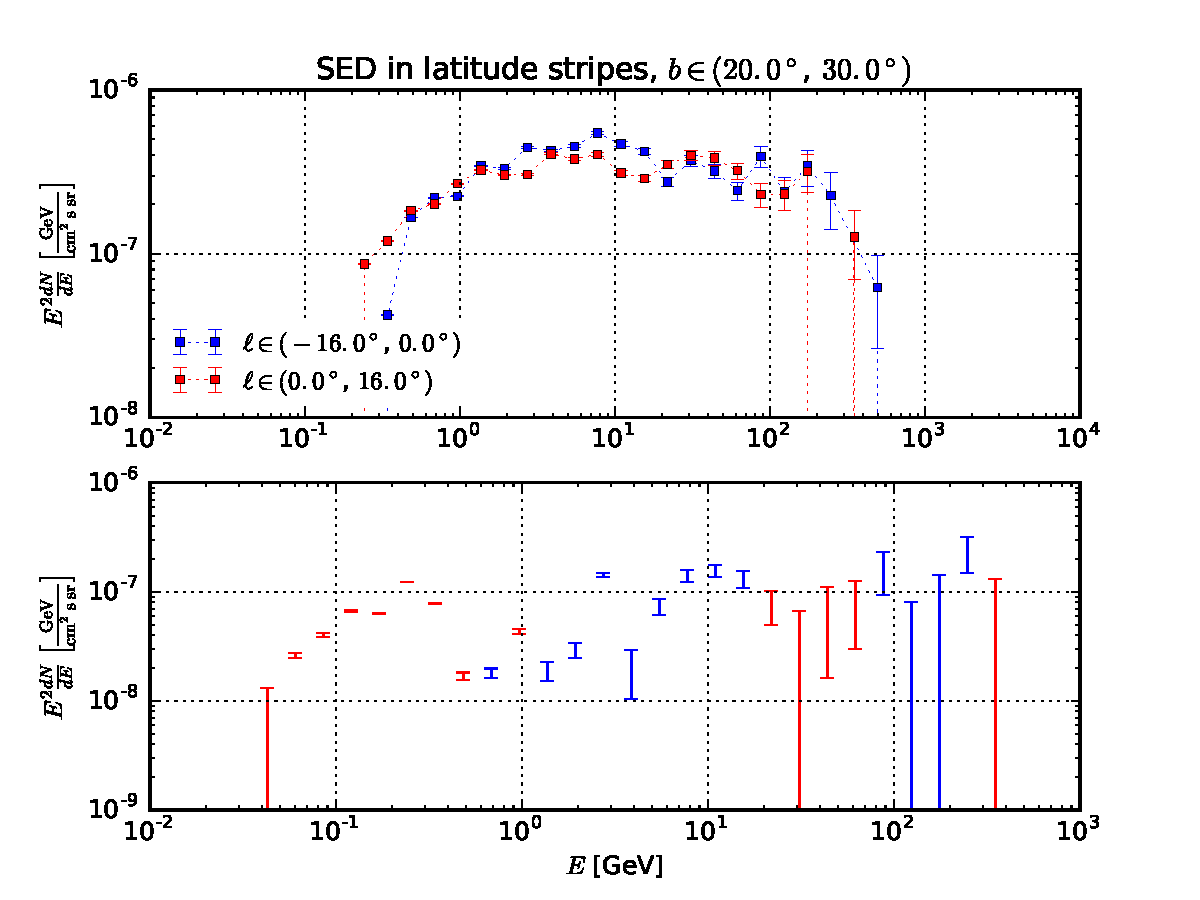
\includegraphics[width=\textwidth]{spectrum_of_top_bubble_in_lat_stripes_20-30.pdf}
    \end{subfigure} 
    \begin{subfigure}{0.5\textwidth}
        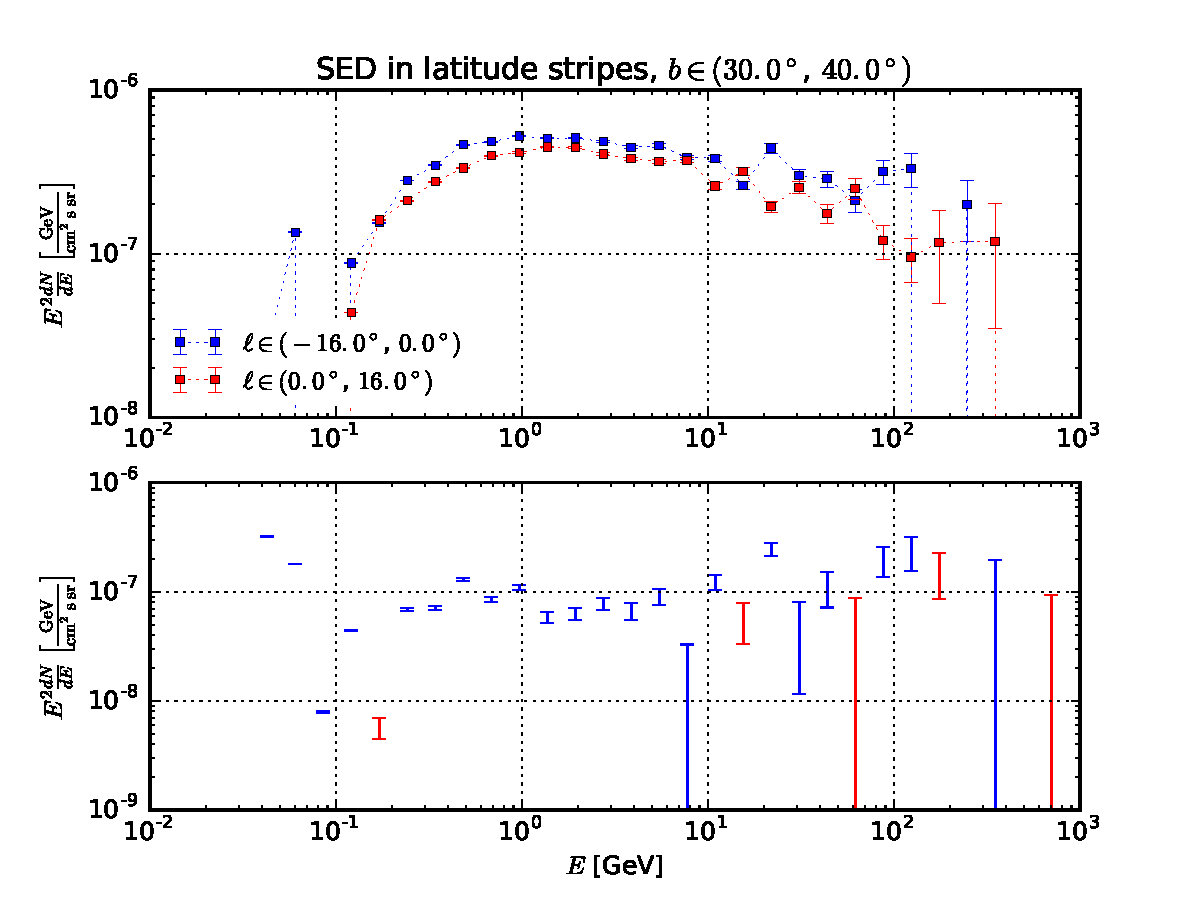
\includegraphics[width=\textwidth]{spectrum_of_top_bubble_in_lat_stripes_30-40.pdf}
    \end{subfigure}
    \begin{subfigure}{0.5\textwidth}
        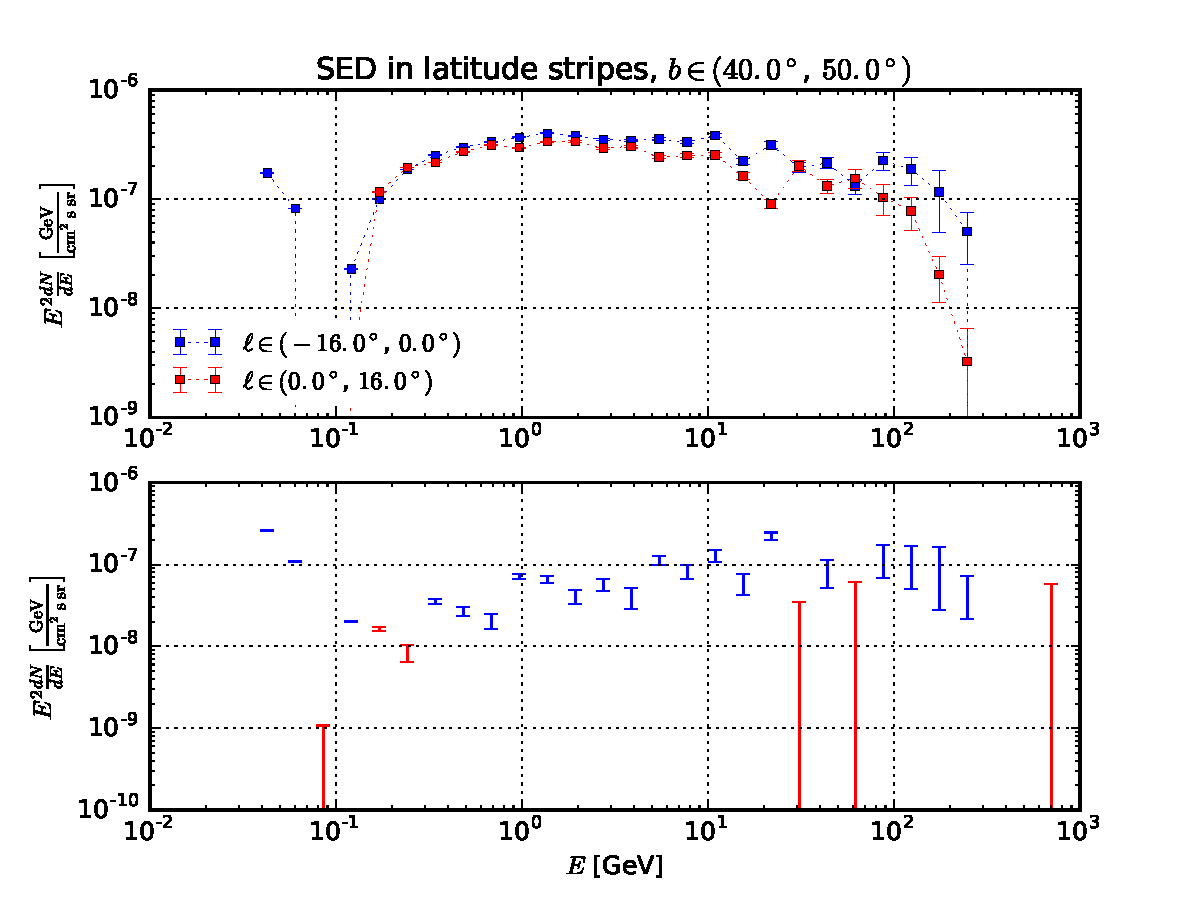
\includegraphics[width=\textwidth]{spectrum_of_top_bubble_in_lat_stripes_40-50.pdf}
    \end{subfigure} 
    \begin{subfigure}{0.5\textwidth}
        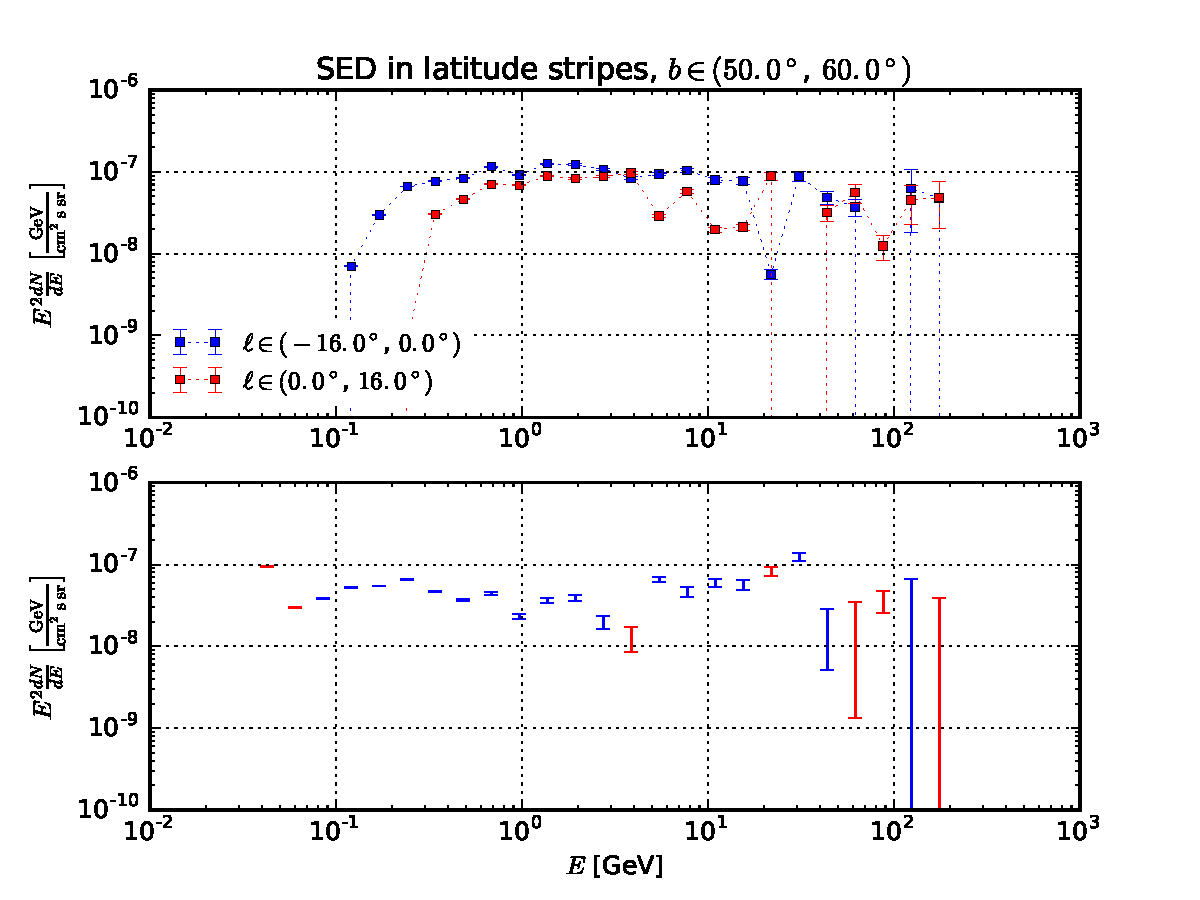
\includegraphics[width=\textwidth]{spectrum_of_top_bubble_in_lat_stripes_50-60.pdf}
    \end{subfigure}
    \caption{Residual SED of northern bubble in $10^\circ$ latitude stripes. The top part of each plot shows the SED east (red) and west (blue). The bottom part illustrates the difference between the SED of east and west, where blue means $\left(E^2\frac{dN}{dE}\right)_\mathrm{west} > \left(E^2\frac{dN}{dE}\right)_\mathrm{east}$ and red the other way round. The $0.5^\circ$ symmetrized mask is used.}
\end{figure}

\begin{figure}
    \begin{subfigure}{0.5\textwidth}
        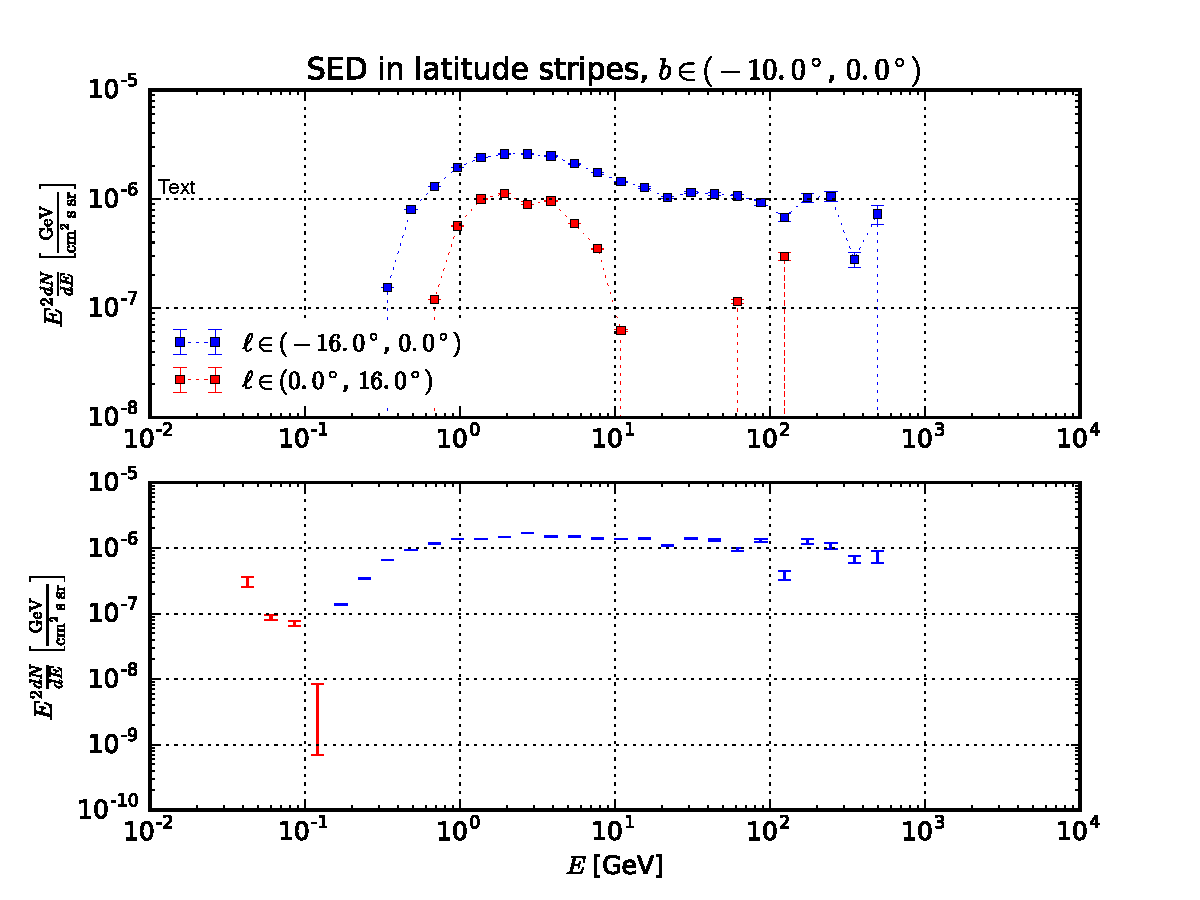
\includegraphics[width=\textwidth]{spectrum_of_bottom_bubble_in_lat_stripes_0-10.pdf}
    \end{subfigure} 
    \begin{subfigure}{0.5\textwidth}
        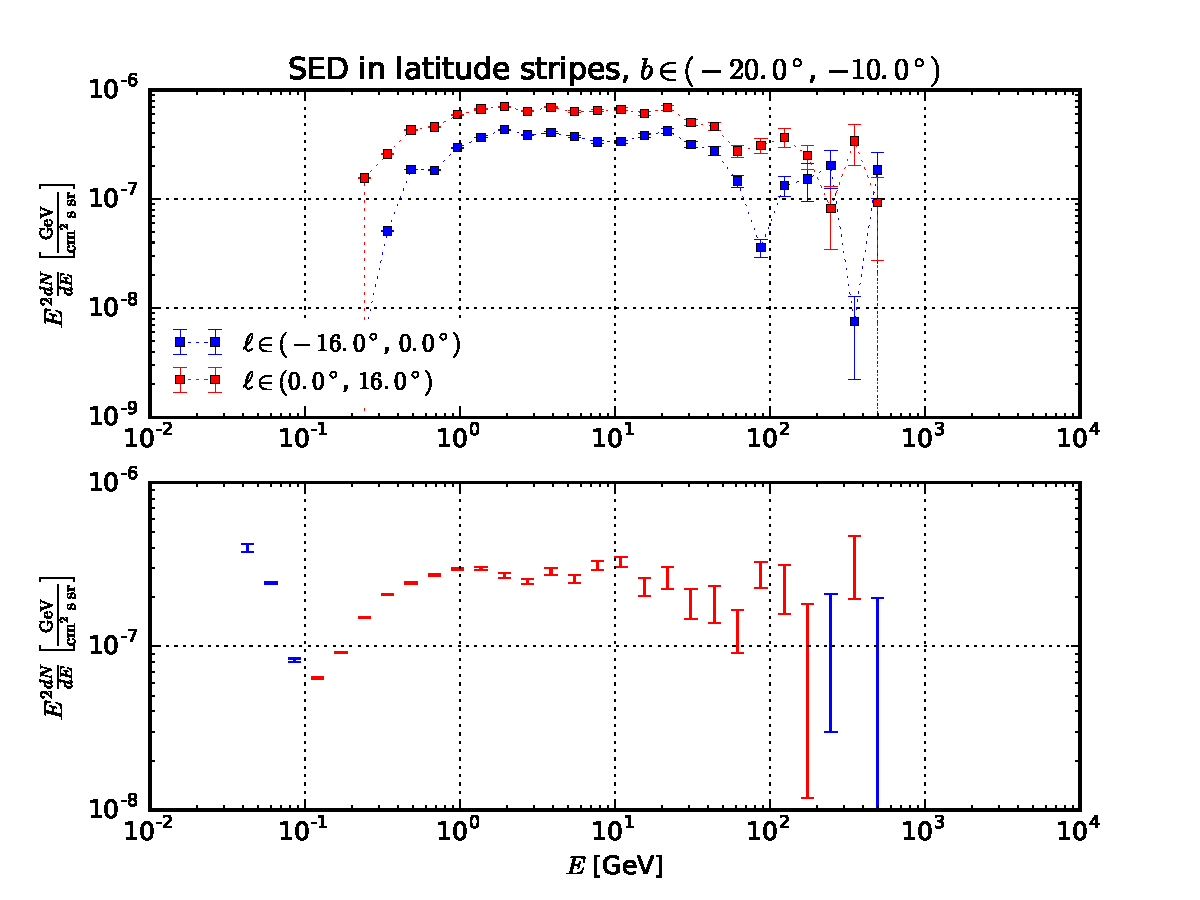
\includegraphics[width=\textwidth]{spectrum_of_bottom_bubble_in_lat_stripes_10-20.pdf}
    \end{subfigure}
    \begin{subfigure}{0.5\textwidth}
        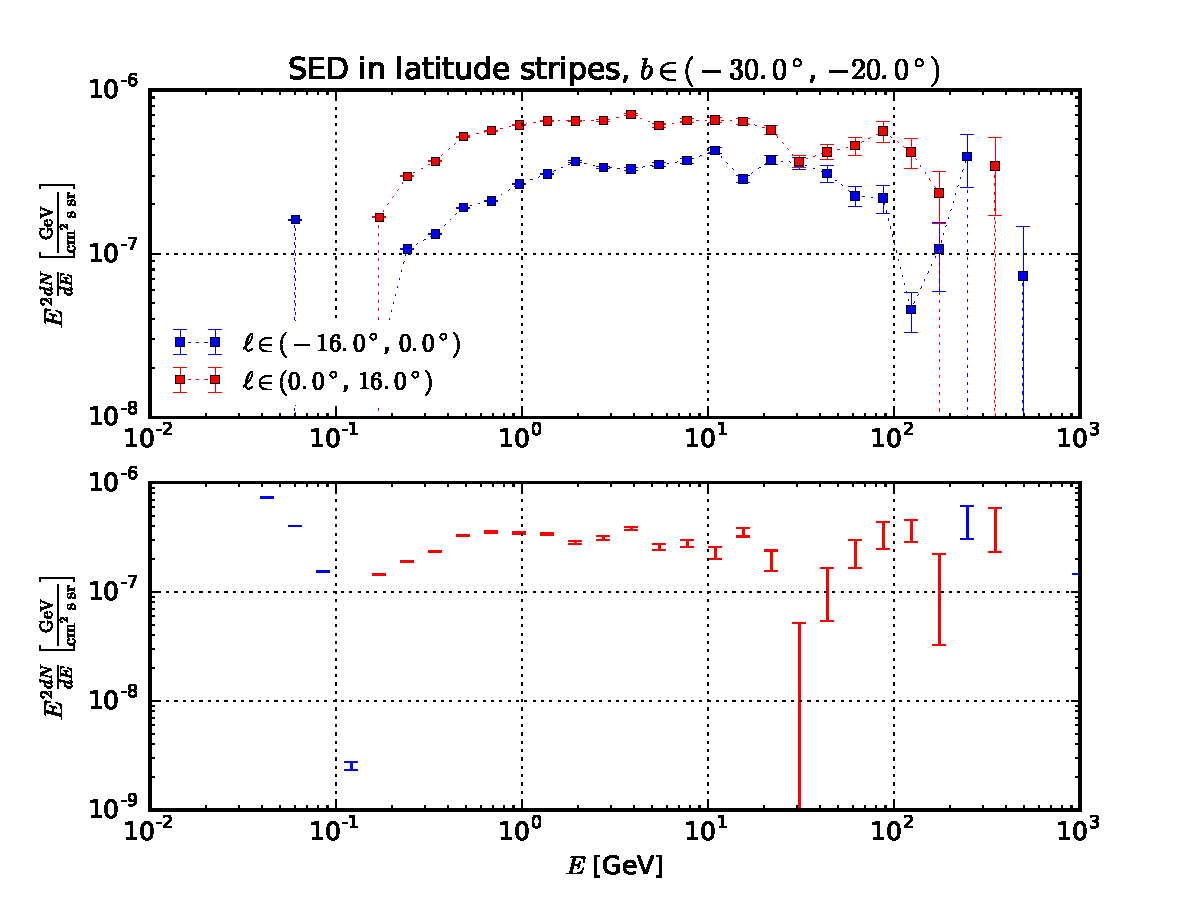
\includegraphics[width=\textwidth]{spectrum_of_bottom_bubble_in_lat_stripes_20-30.pdf}
    \end{subfigure} 
    \begin{subfigure}{0.5\textwidth}
        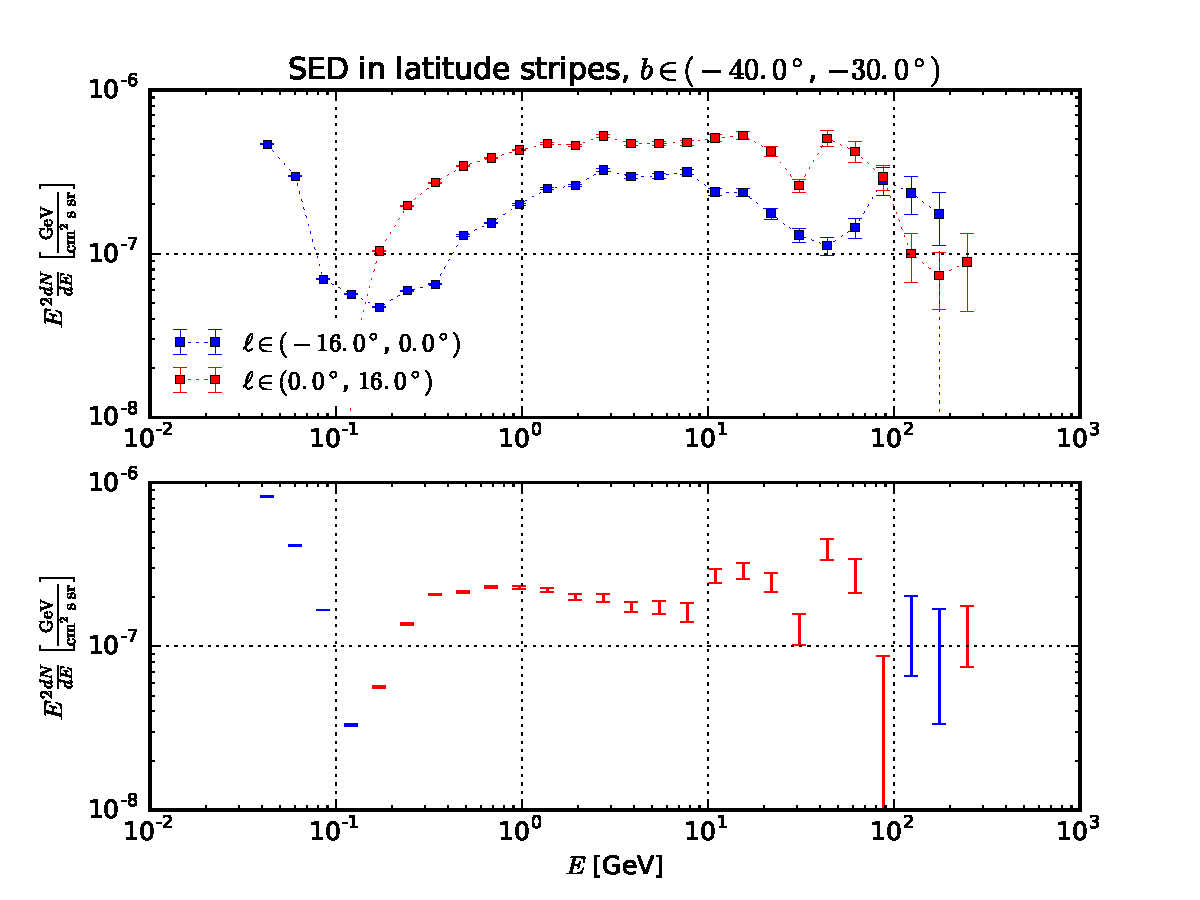
\includegraphics[width=\textwidth]{spectrum_of_bottom_bubble_in_lat_stripes_30-40.pdf}
    \end{subfigure}
    \begin{subfigure}{0.5\textwidth}
        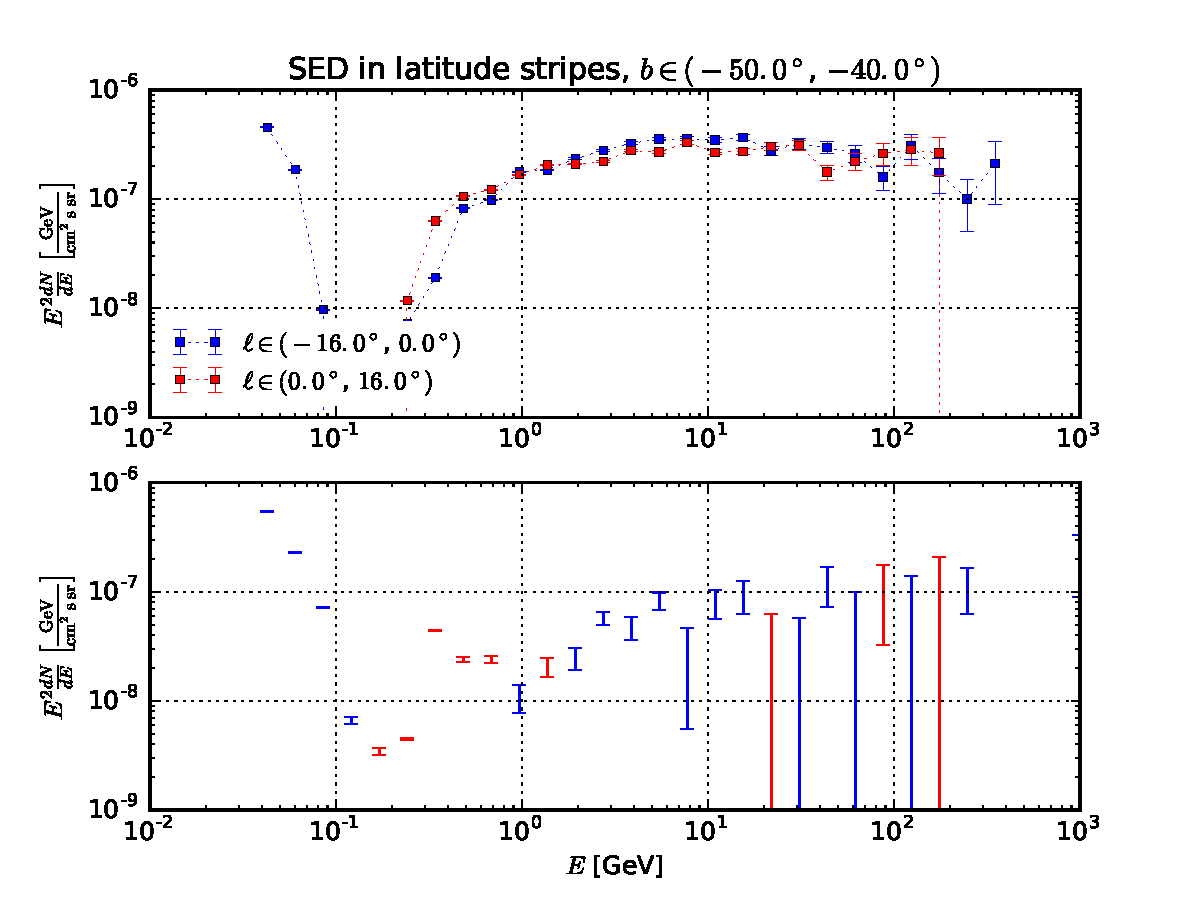
\includegraphics[width=\textwidth]{spectrum_of_bottom_bubble_in_lat_stripes_40-50.pdf}
    \end{subfigure} 
    \begin{subfigure}{0.5\textwidth}
        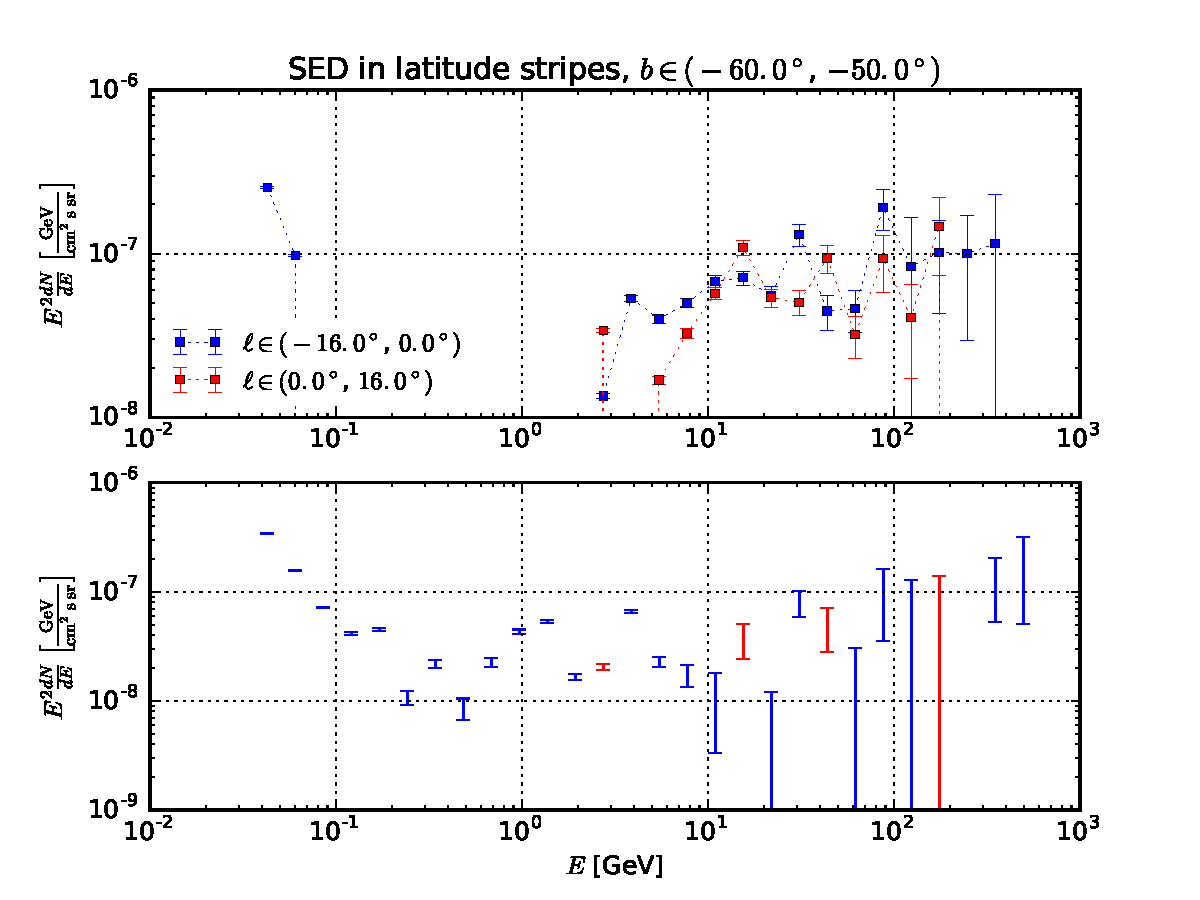
\includegraphics[width=\textwidth]{spectrum_of_bottom_bubble_in_lat_stripes_50-60.pdf}
    \end{subfigure}
    \caption{Same as above but for southern hemisphere.}
\end{figure}


\end{document}
